\newpage
\section{Phương pháp đề xuất}

Đề tài đề xuất một phương pháp dựa trên \textbf{TransReID} kết hợp với cơ chế \textbf{Visibility-Guided Patch Weighting}. Ý tưởng chính là học trọng số cho từng patch đặc trưng để tăng ảnh hưởng của các vùng giàu thông tin nhận dạng và giảm tác động của các vùng bị che khuất, nền phức tạp hoặc ít ổn định giữa các camera.

\subsection{Pipeline}

Ảnh đầu vào trước hết được chia thành các patch và đưa qua backbone Transformer của TransReID để thu được tập đặc trưng patch. Trên các đặc trưng này, một nhánh phụ được thêm vào để dự đoán trọng số cho từng patch. Các trọng số này sau đó được dùng để tái trọng số đặc trưng patch trước khi tổng hợp thành đặc trưng cuối cùng phục vụ cho bài toán nhận dạng lại người.

Pipeline có thể mô tả như sau:
\begin{figure}[H]
    \centering
    \begin{subfigure}[t]{0.48\textwidth}
        \centering
        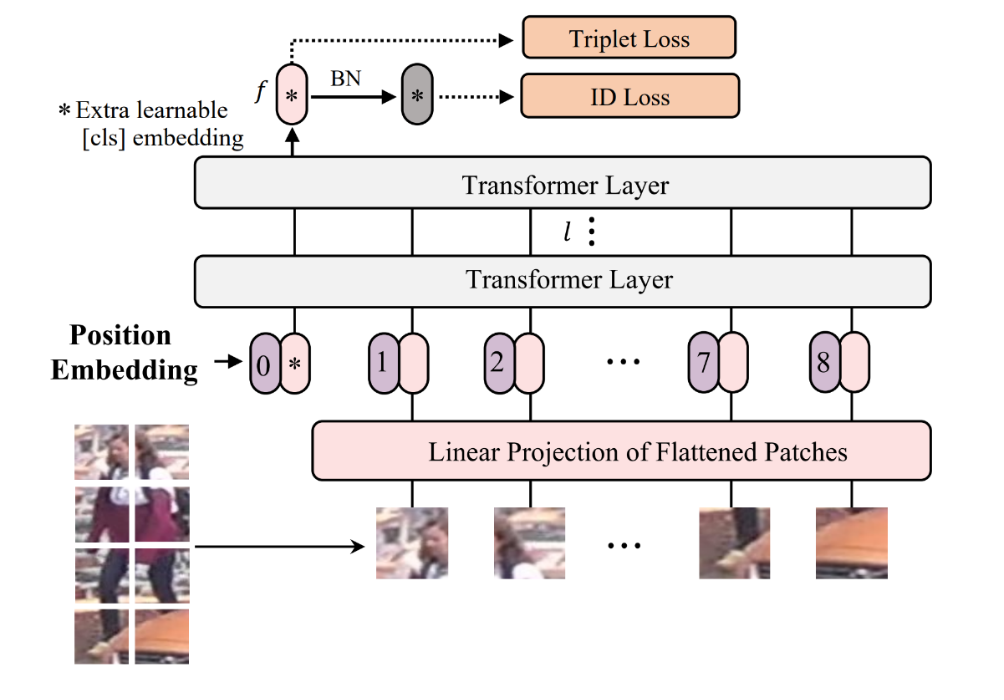
\includegraphics[width=\linewidth]{img/pipeline.png}
        \caption{Mô hình baseline}
        \label{fig:baseline_pipeline}
    \end{subfigure}
    \hfill
    \begin{subfigure}[t]{0.48\textwidth}
        \centering
        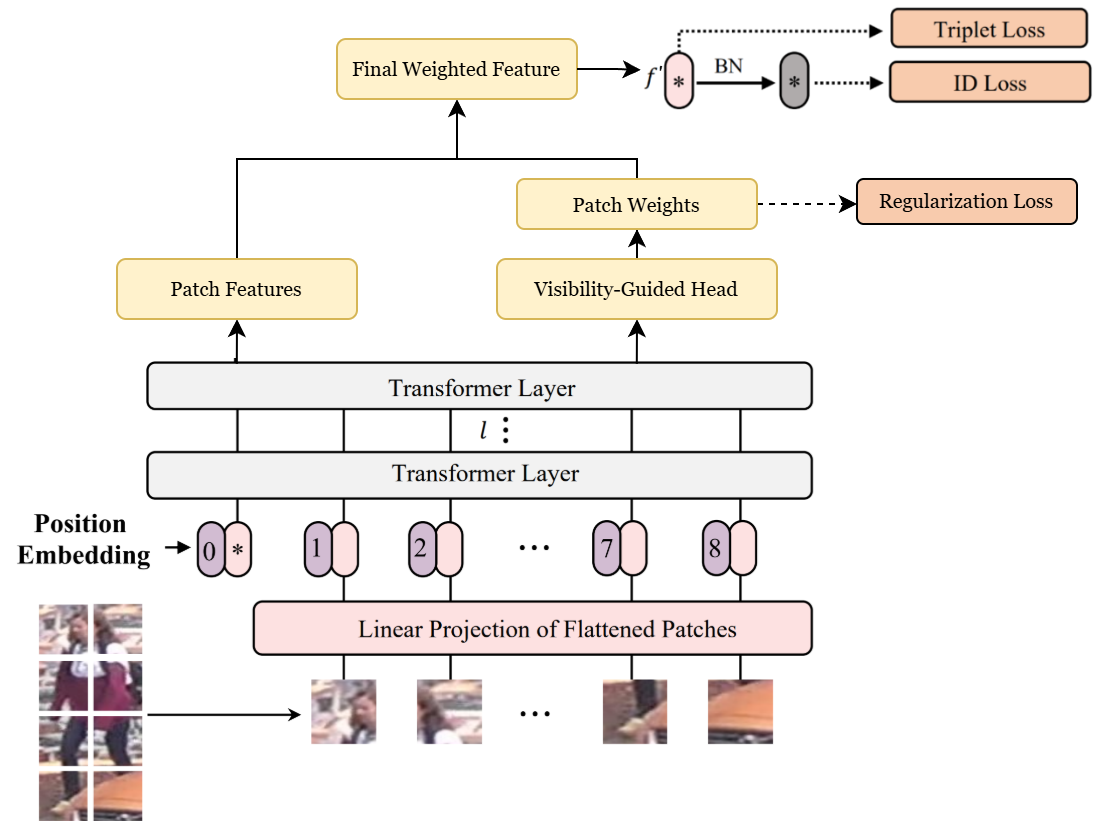
\includegraphics[width=\linewidth]{img/new pipeline.png}
        \caption{Sơ đồ pipeline của phương pháp đề xuất, bao gồm backbone TransReID và cơ chế Visibility-Guided Patch Weighting.}
        \label{fig:new_pipeline}
    \end{subfigure}
    \label{fig:two_pipelines}
\end{figure}

Trong đó, \(f_i\) là đặc trưng của patch thứ \(i\), \(w_i\) là trọng số học được, và \(f_{\text{final}}\) là đặc trưng cuối cùng dùng để truy hồi.

\subsection{Trích xuất đặc trưng}

Backbone TransReID được sử dụng để trích xuất đặc trưng từ ảnh đầu vào dưới dạng các patch embeddings:
\[
F = [f_1,f_2,\dots,f_N], \quad f_i \in \mathbb{R}^d
\]
Để xử lý việc không phải patch nào cũng hữu ích như nhau, đề tài bổ sung một nhánh nhỏ dự đoán trọng số cho từng patch:
\[
w_i = \sigma(\text{MLP}(f_i))
\]
Sau đó, đặc trưng cuối được tính bằng cách tổng hợp các patch đã được tái trọng số:
\[
f_{\text{final}} = \sum_{i=1}^{N} w_i f_i
\]
Cách biểu diễn này giúp mô hình tập trung nhiều hơn vào các vùng đáng tin cậy và giảm ảnh hưởng của các vùng gây nhiễu.

\subsection{Hàm mất mát}
Để huấn luyện mô hình, đề tài sử dụng kết hợp \textbf{ID classification loss} và \textbf{triplet loss}, đồng thời bổ sung một thành phần điều chuẩn cho nhánh weighting nếu cần thiết.

\paragraph{Cross-Entropy Loss} Hàm mất mát phân loại danh tính được dùng để buộc mô hình học đặc trưng có khả năng phân biệt các danh tính khác nhau:
\[
L_{id} = - \sum_{c=1}^{C} y_c \log \hat{y}_c
\]
trong đó \(C\) là số lớp danh tính, \(y_c\) là nhãn thật và \(\hat{y}_c\) là xác suất dự đoán.

\paragraph{Triplet Loss} Để tối ưu trực tiếp quan hệ khoảng cách trong không gian đặc trưng, đề tài sử dụng triplet loss trên đặc trưng cuối \(f_{\text{final}}\). Với anchor \(a\), positive \(p\) và negative \(n\), triplet loss được viết:
\[
L_{tri} = \max \left(0, d(f_a,f_p) - d(f_a,f_n) + m \right)
\]
trong đó \(d(\cdot,\cdot)\) là khoảng cách Euclid và \(m\) là margin. Hàm mất mát này giúp kéo đặc trưng của cùng một người lại gần nhau và đẩy đặc trưng của những người khác ra xa, từ đó cải thiện chất lượng xếp hạng trong truy hồi.

\paragraph{Regularization cho patch weights} Do các trọng số patch được học trực tiếp từ đặc trưng, cần có một cơ chế điều chuẩn để tránh hiện tượng tất cả các patch nhận trọng số gần như nhau hoặc mô hình chỉ tập trung vào rất ít patch. Vì vậy, có thể bổ sung một thành phần điều chuẩn: $L_{reg}$ 
nhằm ổn định quá trình học trọng số và giữ cho cơ chế weighting hoạt động hiệu quả.

Tổng hàm mất mát của mô hình được xác định như sau:
\[
L = L_{id} + \lambda_1 L_{tri} + \lambda_2 L_{reg}
\]
trong đó \(\lambda_1\) và \(\lambda_2\) là các hệ số cân bằng giữa các thành phần mất mát.

Sự kết hợp giữa loss phân loại và loss metric giúp mô hình vừa học được ranh giới danh tính rõ ràng, vừa tối ưu trực tiếp chất lượng truy hồi. Đây là lựa chọn phù hợp cho bài toán person re-identification, trong đó mục tiêu cuối cùng không chỉ là phân loại đúng mà còn là sắp xếp đúng thứ tự tương đồng giữa các ảnh.

\subsection{Tập dữ liệu}
Để đánh giá hiệu quả của phương pháp, thí nghiệm có thể được thực hiện trên các bộ dữ liệu person re-identification phổ biến như \textbf{Market-1501}~\cite{zheng2015market1501} và \textbf{DukeMTMC-reID}~\cite{gou2017dukemtmc4reid}. Đây là các bộ dữ liệu chuẩn, được sử dụng rộng rãi trong nhiều nghiên cứu ReID, cho phép so sánh kết quả một cách công bằng với các phương pháp trước đó.

\begin{itemize}
    \item \textbf{Market-1501}: gồm hơn 32,000 ảnh của 1,501 danh tính được thu thập từ 6 camera. Đây là bộ dữ liệu phổ biến nhất và thường được dùng làm benchmark cơ bản.
    \item \textbf{DukeMTMC-reID}: gồm hơn 36,000 ảnh của 1,404 danh tính từ 8 camera, có mức độ đa dạng lớn hơn về góc nhìn và điều kiện quan sát.
\end{itemize}

Trong phạm vi đề tài, có thể ưu tiên sử dụng \textbf{Market-1501} làm tập dữ liệu chính để xây dựng và kiểm chứng ý tưởng, sau đó mở rộng đánh giá trên \textbf{DukeMTMC-reID} nếu điều kiện thời gian và tài nguyên cho phép. Cách lựa chọn này giúp cân bằng giữa tính khả thi khi triển khai và giá trị học thuật của thí nghiệm.

\subsection{Phương pháp đánh giá}

Hiệu quả của mô hình được đánh giá bằng các chỉ số chuẩn trong bài toán person re-identification, bao gồm \textbf{CMC} và \textbf{mAP}.

\begin{itemize}
    \item \textbf{Rank-1, Rank-5, Rank-10}: phản ánh khả năng ảnh đúng xuất hiện trong top-\(k\) kết quả truy hồi.
    \item \textbf{mAP}: đánh giá chất lượng xếp hạng tổng thể, là chỉ số đặc biệt quan trọng trong bài toán ReID.
\end{itemize}

Ngoài ra, cần thực hiện \textbf{ablation study} để so sánh giữa mô hình TransReID gốc và mô hình đề xuất có thêm cơ chế Visibility-Guided Patch Weighting. Kỳ vọng chính của phương pháp là cải thiện \textbf{mAP} rõ hơn \textbf{Rank-1}, do cơ chế đề xuất tác động trực tiếp đến chất lượng biểu diễn và thứ tự truy hồi.